\chapter{Analysis of Performance}

\section{Test Objectives}
The test campaigns presented here aim to investigate the performance of UDP communication in a local network under conditions similar to those in a distributed test support system. The considered performance indicators are latency and jitter. The investigations are performed using the star topology with the iHawk in the center, presented in \ref{chap:TopoiHawk}.

There are several factors that can contribute to the latency of a network. However, since there are no intermediate stations between the computer systems in the network topology, the focus will be on these computer systems and their operating states. In a computer system, latency is influenced by the network interface and driver, processing in the network stack, and the application.

The worst-case latency (see \ref{chap:LatencyExplanation}) is the most important indicator for these investigations. However, the mean latency should be also considered. Additionally, secondary data, such as packet losses and datagram sequence, are taken into consideration.

\section{System under Test}
Although the topology with the iHawk in the center is used, in contrast to the reliability tests with this topology (see \ref{chap:ReliabIhawk}), not all bi-directional links between the iHawk in the center and the High-Performance or Traffic PCs are to be examined simultaneously. Instead, a single isolated communication is considered.

\begin{figure}[h]
    \centering
    \begin{subfigure}[b]{0.45\textwidth}
        \centering
        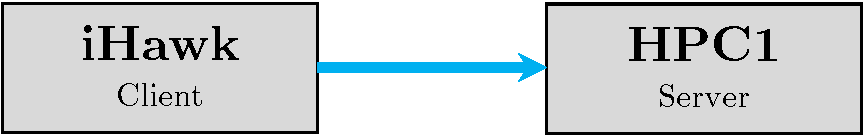
\includegraphics[width=\textwidth]{figures/performance/sut_1a.pdf}
        \caption{Direction 'H'}
        \label{fig:SutHpcPerf:H}
    \end{subfigure}
    \hfill
    \begin{subfigure}[b]{0.45\textwidth}
        \centering
        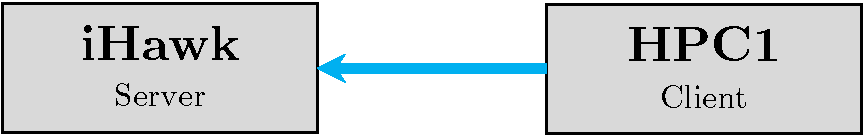
\includegraphics[width=\textwidth]{figures/performance/sut_1b.pdf}
        \caption{Direction 'R'}
        \label{fig:SutHpcPerf:R}
    \end{subfigure}
    \caption{Illustration of the used System under Test with a High-Performance PC.}
    \label{fig:SutHpcPerf}
\end{figure}

The system under test is defined as the UDP communication generated by the TestSuite. Figure  \ref{fig:SutHpcPerf} illustrates this communication between the iHawk and HPC1. Both directions are considered in the campaigns. Direction '\textbf{H}', as depicted in Figure \ref{fig:SutHpcPerf:H}, refers to the communication with iHawk as the sender and HPC1 as the receiver. In contrast, Figure \ref{fig:SutHpcPerf:R} illustrates Direction '\textbf{R}', where HPC1 acts as the sender and iHawk as the receiver.

Similarly, a UDP communication between the iHawk and TPC1 was also considered a system under test. Again, both directions were analyzed.

The network interfaces mentioned in the topology description are used unless otherwise stated in the test campaign description. Furthermore, as with the reliability tests with the iHawk in the center, several settings recommended in the Intel Linux Performance Tuning Guide for the Ethernet 700 series were used. A list of these settings can be found in chapter \ref{chap:ReliabIhawk:SuT}.

\section{Accuracy of Measurements}
As demonstrated in \ref{chap:LatencyExplanation}, latency calculation is based on the difference between two time stamps. One of them is recorded at the sender and the other at the receiver. In order to calculate a valid latency value, clock synchronization between the systems is required. The accuracy and reliability of the measurements depend on the accuracy of this clock synchronization.

The Precision Time Protocol (PTP) is utilized to synchronize clocks between the systems. PTP, as defined in IEEE 1588-2008 \cite{perf01}, synchronizes distributed clocks in a network using the master-slave principle. The master sends messages with synchronization information, enabling all slaves to synchronize their internal clocks with the master. The protocol is also able to handle time delays introduced by the network.

The programs ptp4l and phc2sys implement the PTP standard for Linux. They provide information about the accuracy of the synchronization with the master offset \cite{perf02}. Table \ref{tab:PTPMasterOffset} shows this information for the setup used in the test. HPC1 was the master and TPC1 and the iHawk were the slaves.

\begin{table}[h]
\centering
\begin{tabular}{lll}
	\toprule
	System & Role & Master Offset \\
	\midrule
 	HPC1 & Master & - \\ 
 	TPC1 & Slave & ±80 ns \\
 	iHawk & Slave & ±85 ns \\
	\bottomrule
\end{tabular}
\caption{PTP Master Offset in the Test Setup.}
\label{tab:PTPMasterOffset}
\end{table}

The data indicates that the clocks of the two slaves synchronize with the master with an accuracy of 80 to 85 ns. Since the measured latencies in the test are expected to be at least in the two- to three-digit microsecond range, the accuracy of the clock synchronization is sufficient to provide reliable latency results.

\section{Test Campaigns}

\subsection{Tests with UDP, Raw and Packet Sockets} \label{chap:PerfSockType}
\subsubsection{Motivation and Context}
The purpose of this test campaign is to examine and compare the latency of UDP, Raw, and Packet sockets. Both the sender and receiver will use the respective socket type. No additional system load will be applied to either computer system.

The test campaigns will be carried out with datagram sizes ranging from 80 to 8080 bytes, increasing in steps of 1000 bytes. Additionally, a datagram size of 65000 bytes was tested for UDP sockets utilizing fragmentation.

All tests were conducted using the iHawk and HPC1 systems under test, with a cycle time of 0 µs used, which corresponds to an uninterrupted transmission process. The test duration for each datagram size was 60 seconds.

\subsubsection{Results}
\paragraph{Worst-Case Latency}

\begin{figure}[h]
  \centering
  \subcaptionbox{Direction 'H'\label{fig:SockTypeWc:a}}{%
    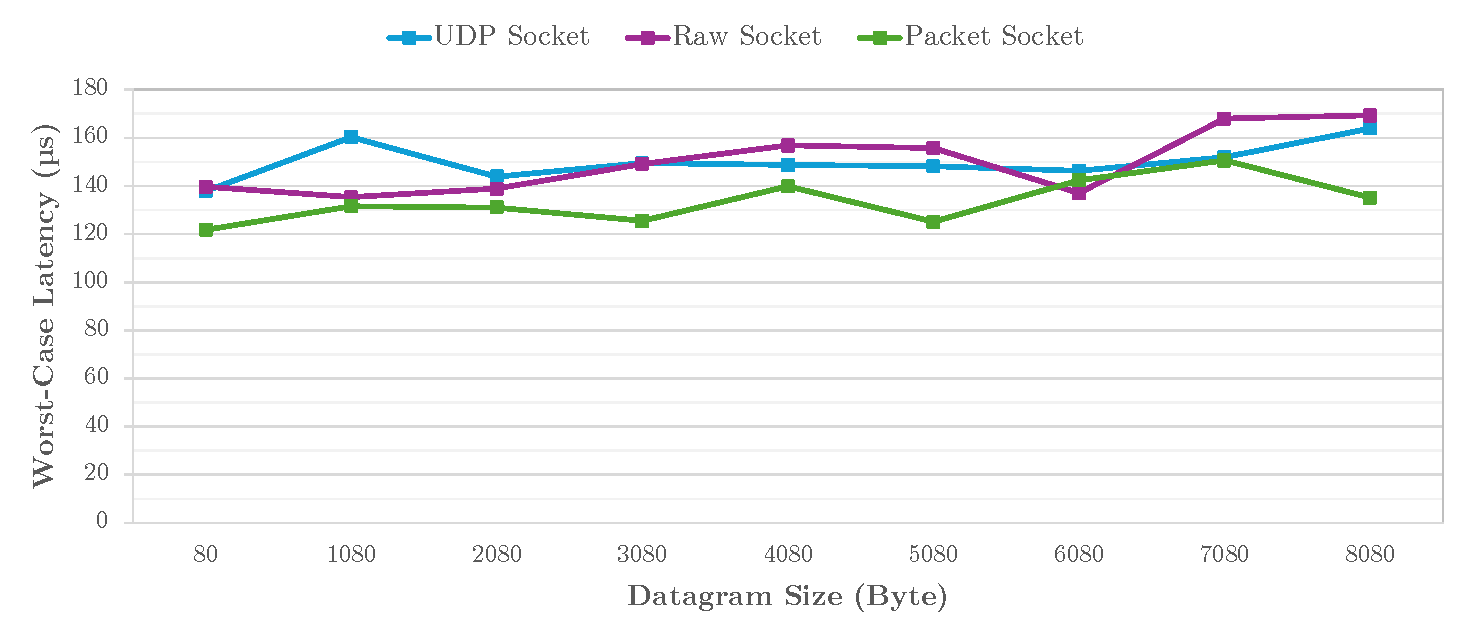
\includegraphics[width=1\textwidth]{figures/performance/d_2a.pdf}
  }
  \subcaptionbox{Direction 'R'\label{fig:SockTypeWc:b}}{%
    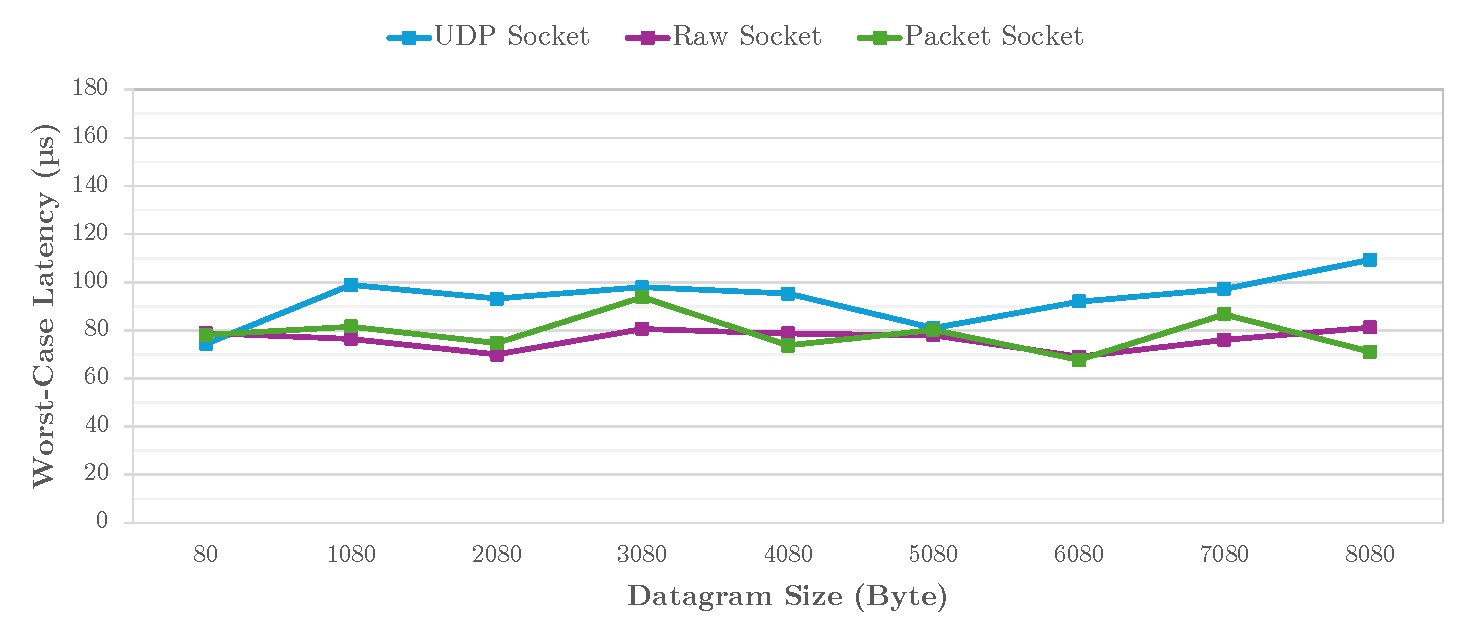
\includegraphics[width=1\textwidth]{figures/performance/d_2b.pdf}
  }
  \caption{Worst-Case Latency by Datagram Size and Socket Type (Campaign 'Tests with UDP, Raw and Packet Sockets').}
  \label{fig:SockTypeWc}
\end{figure}

Figure \ref{fig:SockTypeWc} displays the worst-case latency for the three investigated socket types in relation to the datagram size. A distinction is made between direction 'H' and 'R'.

The worst-case latency for UDP sockets in the 'H' direction is 163.97 µs, while Raw sockets have a slightly higher worst-case latency of 169.32 µs. Packet sockets, on the other hand, have a slightly lower worst-case latency of 150.61 µs. Figure \ref{fig:SockTypeWc:a} illustrates the worst-case latency as in relation of datagram size. The figure shows that the worst-case latency fluctuates, but no trend is apparent from the data.

The worst-case latency in direction 'R' is significantly lower than in direction 'H'. When using UDP sockets, the worst-case latency is 109.31 µs, with Raw sockets it is 81.19 µs, and with Packet sockets it is 93.87 µs. Figure \ref{fig:SockTypeWc:b} displays the worst-case latency as a function of datagram size, but again no trend can be identified.

It is noticeable that the measured worst-case latency in the 'R' direction is 33\% lower than in the 'H' direction when using UDP sockets. This reduction is even greater at 52\% when using Raw sockets. The exact reason for this difference is difficult to determine at this point due to the inability to obtain time stamps from the network interface, which makes it impossible to identify which system causes how much latency. Both systems use the same network interface, so a likely cause of these differences between the 'H' and 'R' directions is the different hardware of the systems.

When examining the time distribution of latencies, it is evident that the highest latencies (worst-case latencies) consistently occur for the first 10 packets sent during the test. This applies to all socket types in both directions. As previously mentioned, no time stamps can be obtained from the network interface, making it difficult to analyze the reason for this observation.

During the tests, no packet losses were detected with any of the three socket types examined. However, it was found that when Packet sockets are used in both the 'H' and 'R' directions, the packets are re-sorted and do not arrive in the correct order. This behavior was not observed with UDP sockets and Raw sockets.

\paragraph{Mean Latency}

Figure \ref{fig:SockTypeMl} shows the mean latency for different datagram sizes, compared across the three examined socket types.

\begin{figure}[h!]
  \centering
  \subcaptionbox{Direction 'H'\label{fig:SockTypeMl:a}}{%
    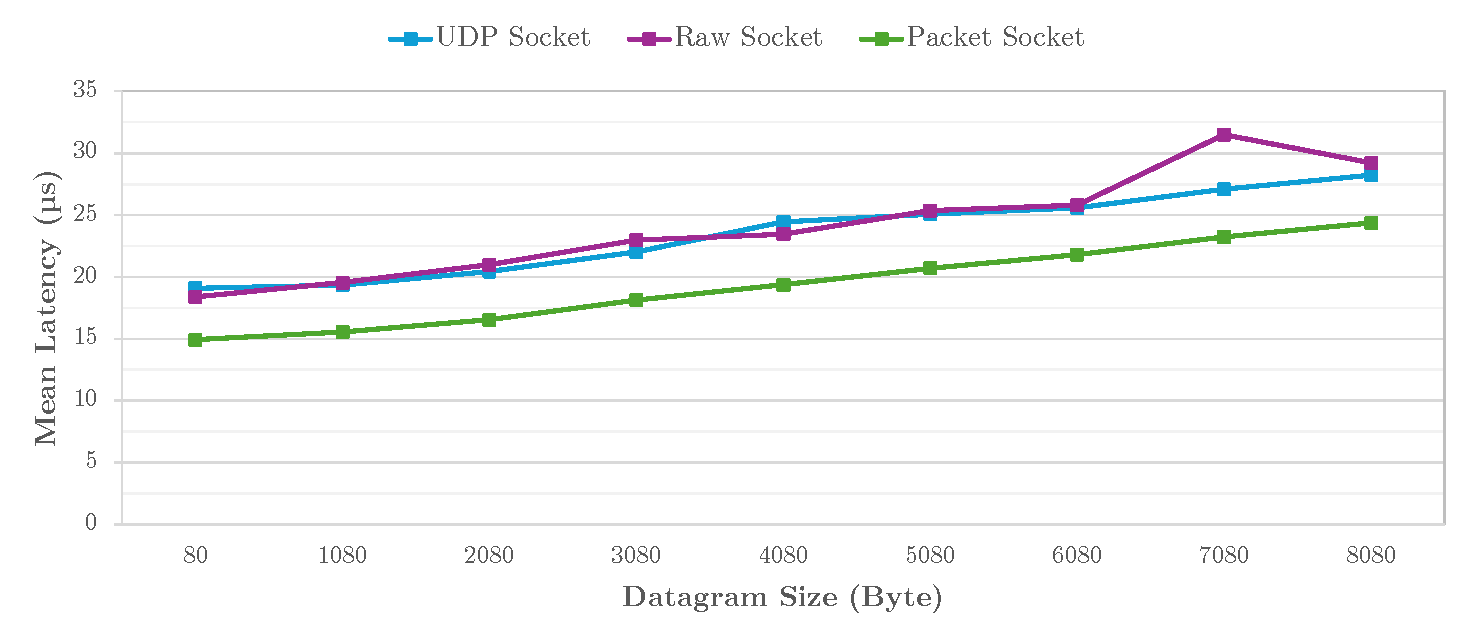
\includegraphics[width=1\textwidth]{figures/performance/d_3a.pdf}
  }
  \subcaptionbox{Direction 'R'\label{fig:SockTypeMl:b}}{%
    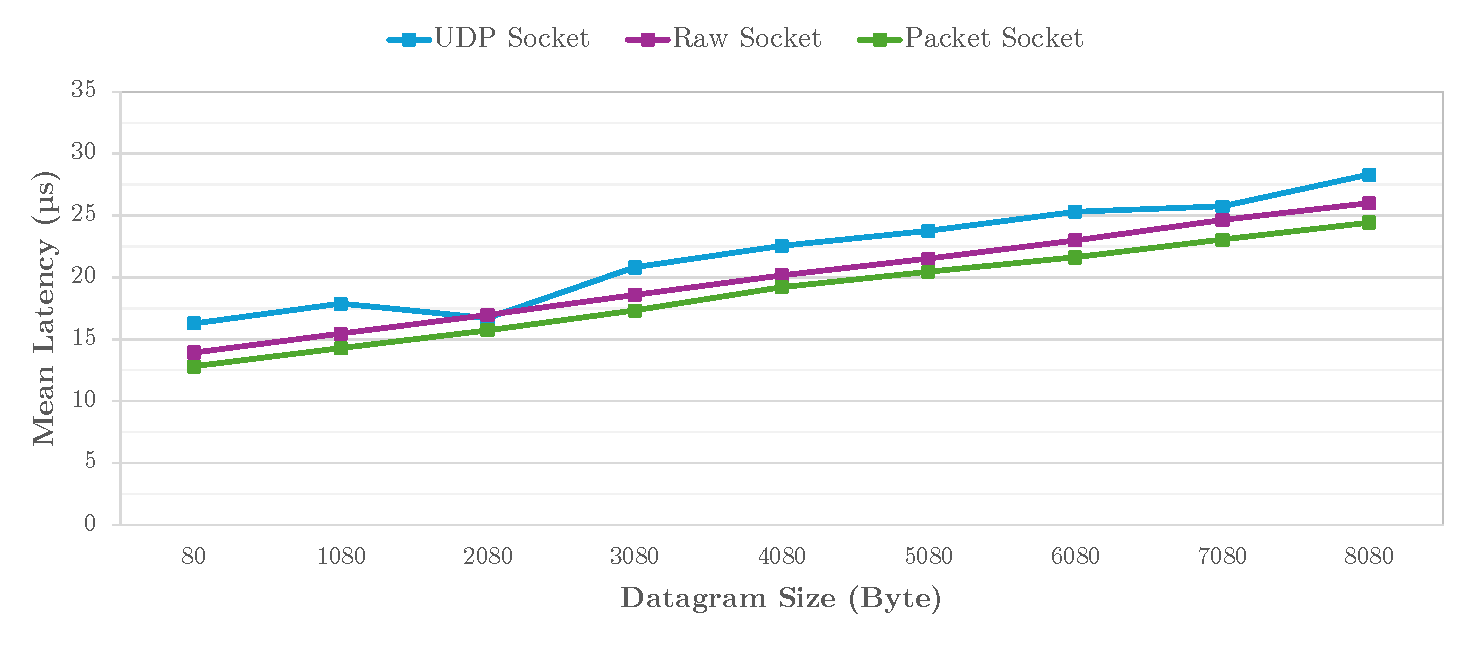
\includegraphics[width=1\textwidth]{figures/performance/d_3b.pdf}
  }
  \caption{Mean Latency by Datagram Size and Socket Type (Campaign 'Tests with UDP, Raw and Packet Sockets').}
  \label{fig:SockTypeMl}
\end{figure}

In the direction 'H', the mean latency is 26.4 µs across all datagram sizes when using UDP sockets. Raw socket have has a comparable mean latency of 27.15 µs. Packet sockets had the lowest mean latency of 21.83 µs, which is 17\% lower than UDP sockets.

Figure \ref{fig:SockTypeMl:a} illustrates the correlation between datagram size and mean latency. The data indicates that as the size of the datagram increases, the mean latency also increases. This is primarily due to the fact that larger packets require more processing.

In the direction 'R', UDP sockets had a mean latency of 24.67 µs. Raw sockets and Packet sockets had a mean latency that was approximately 10\% lower, as shown in Figure \ref{fig:SockTypeMl:b}. The figure also demonstrates that the mean latency increases also in this direction when the datagram size is increased. The mean latency in the 'R' direction is lower than that in the 'H' direction.

\paragraph{Influence of Fragmentation on Latency}

The campaign also examined the latency associated with fragmentation, using a datagram size of 65000 bytes as an example. The test was only performed with UDP sockets, as Raw and Packet sockets do not support fragmentation.

\begin{figure}[h!]
  \centering

  \begin{subfigure}[b]{0.45\linewidth}
    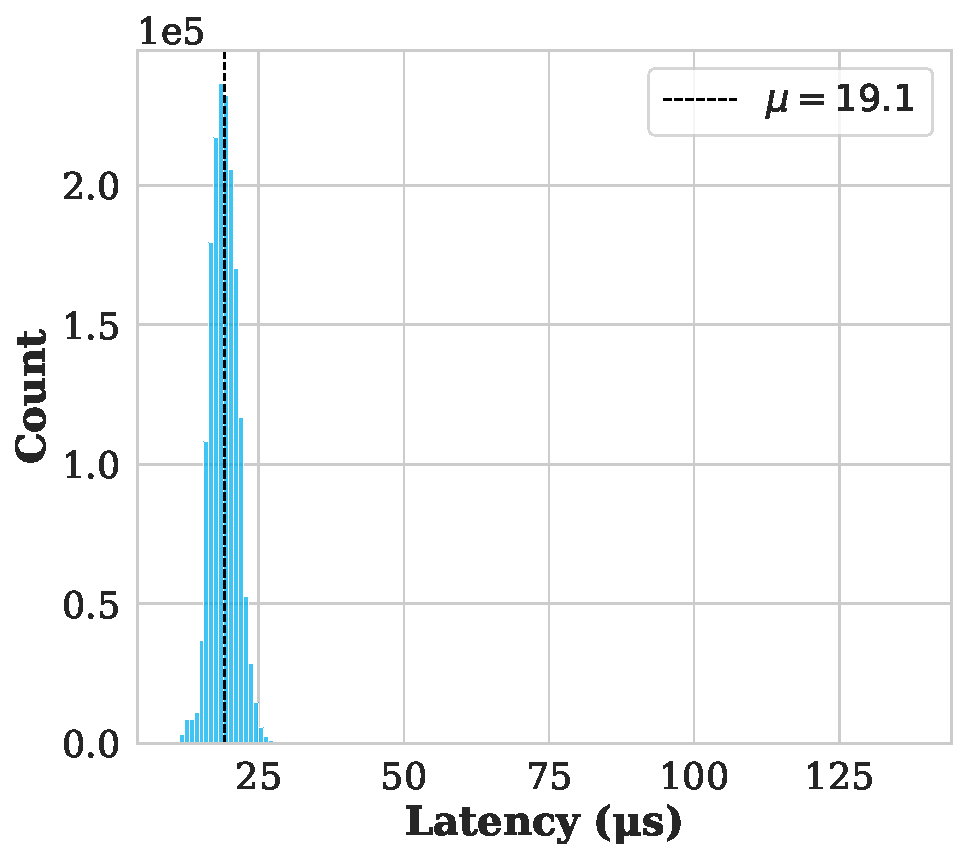
\includegraphics[width=\linewidth]{figures/performance/d_4a.pdf}
    \caption{80 Byte}
    \label{fig:histFrag:a}
  \end{subfigure}
  \hfill
  \begin{subfigure}[b]{0.45\linewidth}
    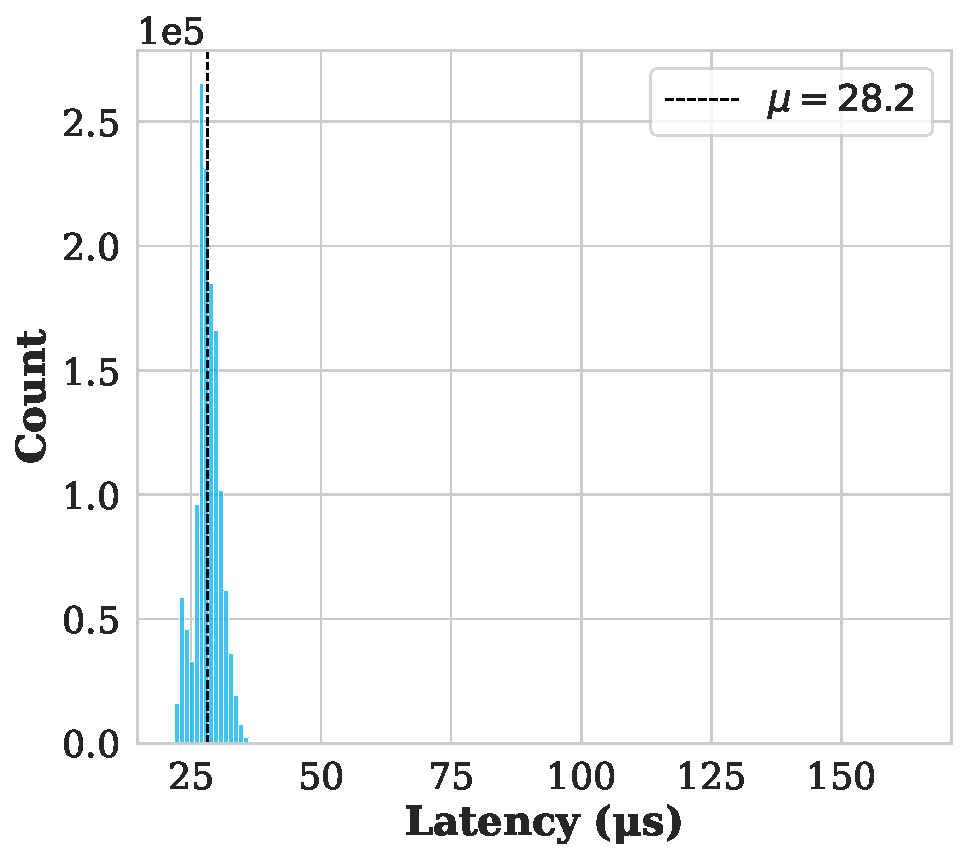
\includegraphics[width=\linewidth]{figures/performance/d_4b.pdf}
    \caption{8900 Byte}
    \label{fig:histFrag:b}
  \end{subfigure}

  \begin{subfigure}[b]{0.45\linewidth}
    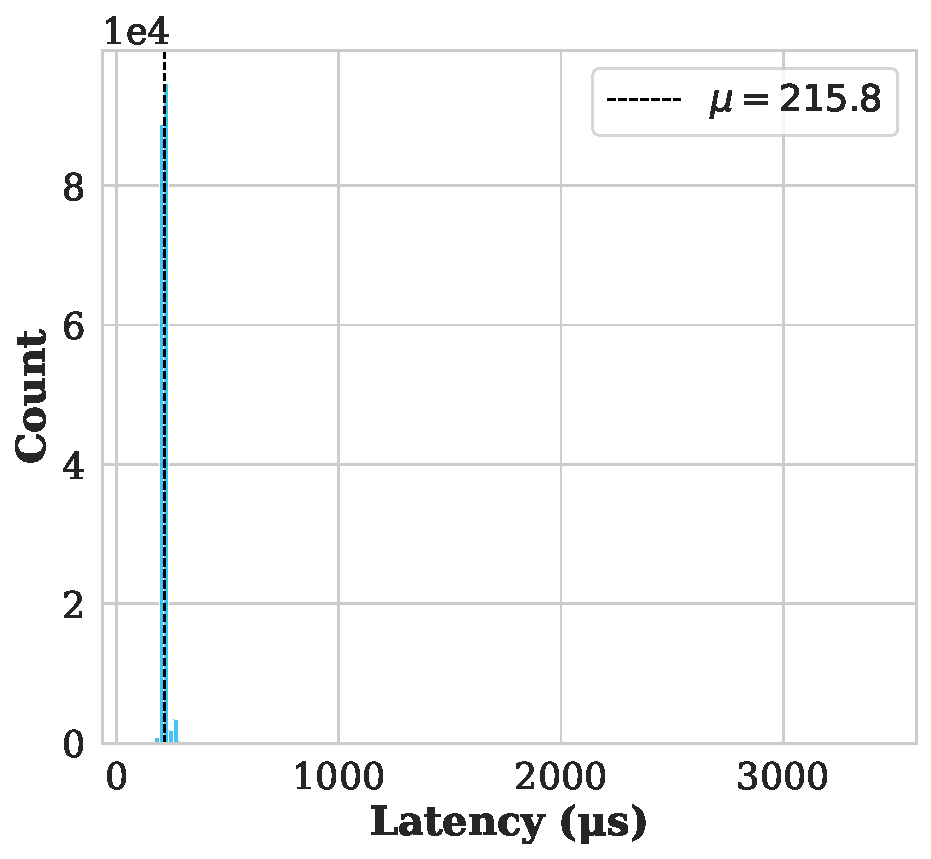
\includegraphics[width=\linewidth]{figures/performance/d_4c.pdf}
    \caption{65000 Byte}
    \label{fig:histFrag:c}
  \end{subfigure}
  \hfill
  \begin{subfigure}[b]{0.45\linewidth}
    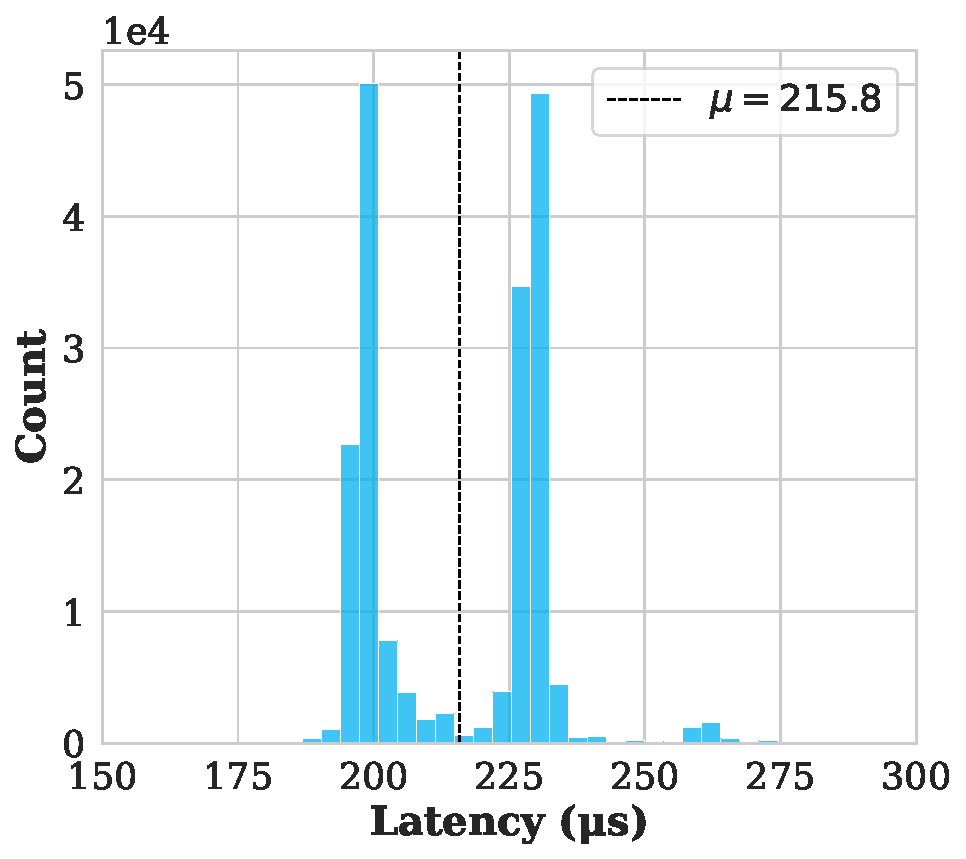
\includegraphics[width=\linewidth]{figures/performance/d_4d.pdf}
    \caption{65000 Byte (enlarged Section)}
    \label{fig:histFrag:d}
  \end{subfigure}
  
  \caption{Latency Distribution for UDP Sockets with different Datagram Sizes in Direction 'H' (Campaign 'Tests with UDP, Raw and Packet Sockets').}
  \label{fig:histFrag}
\end{figure}

Figure \ref{fig:histFrag} displays histograms of the latency for datagram sizes of 80 bytes, 8900 bytes and 65000 bytes in direction 'H'. Figure \ref{fig:histFrag:d} presents an enlarged version of the histogram, showing only the section from 150 µs to 300 µs.

With a datagram size of 65000 bytes (see Figure \ref{fig:histFrag:c}), a worst case latency of 3431.16 µs was observed, which is more than 20 times higher than with a datagram size of 8900 bytes (163.97 µs). The mean latency for a datagram size of 65000 bytes is 215.78 µs, which is approximately 7.5 times higher than for a datagram size of 8900 bytes. This difference can be attributed to fragmentation (see \ref{chap:frag}). When a UDP datagram with a size of 65000 bytes is sent, it is divided into 8 packets at an MTU of 9000 bytes. This correlates with the observed increase in mean latency.

While the distribution is close to the mean for datagram sizes of 80 bytes (see Figure \ref{fig:histFrag:a}) and 8900 bytes (see Figure \ref{fig:histFrag:b}), a wider distribution can be seen for a datagram size of 65000 bytes. Upon closer inspection of the enlarged section in Figure \ref{fig:histFrag:d}, a multimodal distribution is observed.

Additionally, it was discovered that datagrams are rearranged at a datagram size of 65000 bytes due to fragmentation.  These fundamental observations about fragmentation also apply to direction 'R'.

\subsubsection{Classification of Results}
One outcome of this campaign is that Packet have a lower worst-case and mean latency than UDP sockets or Raw sockets, but it was observed as a secondary result observed that packets do not arrive in the application in the order in which they were sent. Another argument against Packet sockets is that they are more complex to handle, since layer 2, 3, and 4 headers must be generated by the application. For this reason, this Socket Type will not be considered in the further performance analysis.

The campaign also revealed that Raw sockets have a latency comparable to that of UDP sockets. However, they are also more complex to handle than UDP sockets, so they are not considered in the following campaigns.

Regarding fragmentation, the campaign discovered that latency increases significantly for datagram sizes above the MTU due to fragmentation. Additionally, it was observed that fragmented packets arrive in reverse order.


\subsection{Tests using the System under Test with a Traffic PC}

\subsubsection{Motivation and Context}
The purpose of this test campaign is to examine the latency of the system under test utilizing the iHawk and a Traffic PC. Both directions 'H' and 'R' are considered.

Based on the results of the previous test campaign 'Tests with UDP, Raw and Packet Sockets' (see \ref{chap:PerfSockType}), the tests were performed only with UDP sockets and datagram sizes from 80 to 8080 bytes in steps of 1000 bytes. The cycle time and test duration used in this campaign are the same as in the previous one.

\subsubsection{Results}
\paragraph{Worst-Case Latency}

\begin{figure}[h!]
  \centering
  \subcaptionbox{Direction 'H'\label{fig:TrafficWc:a}}{%
    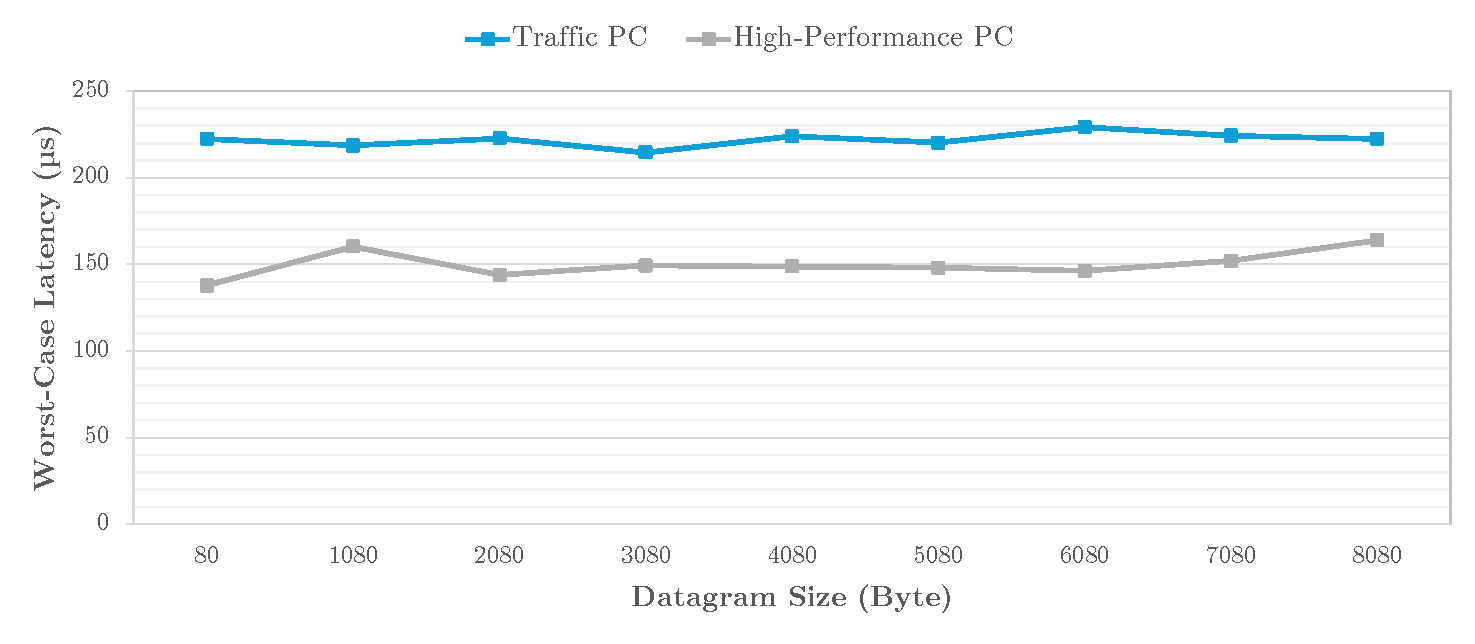
\includegraphics[width=1\textwidth]{figures/performance/d_5a.pdf}
  }
  \subcaptionbox{Direction 'R'\label{fig:TrafficWc:b}}{%
    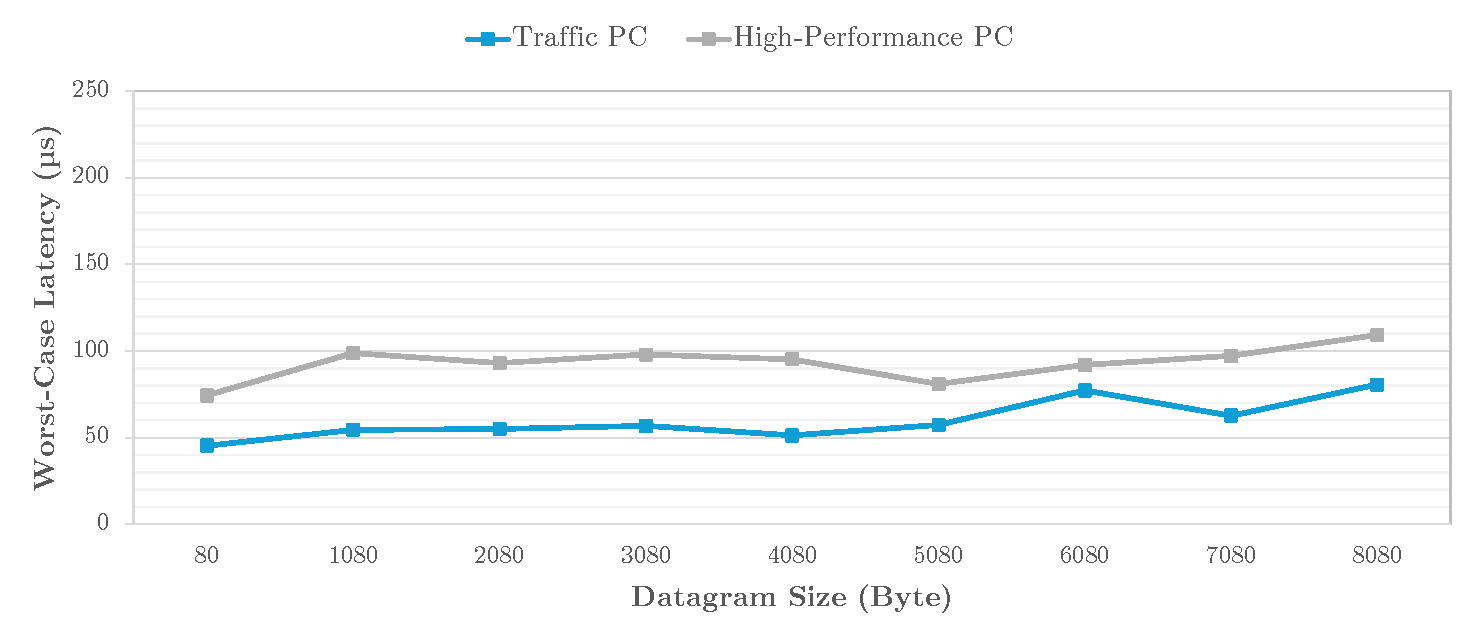
\includegraphics[width=1\textwidth]{figures/performance/d_5b.pdf}
  }
  \caption{Worst-Case Latency by Datagram Size and System under Test (Campaign 'Tests using the System under Test with a Traffic PC').}
  \label{fig:TrafficWc}
\end{figure}

Figure \ref{fig:TrafficWc} displays the worst-case latency for the system under test with a Traffic PC. Additionally, the results from the previous test campaign (see \ref{chap:PerfSockType}) for a UDP socket with a high performance PC as the system under test are shown for comparison.

In direction 'H' a worst case latency of 229.20 µs was measured. Figure \ref{fig:TrafficWc:a} shows it in relation to the datagram size. The worst-case latency of the system under test with a Traffic PC is therefore approximately 30\% higher than with a High Performance PC.

Possible reasons for the higher latency in the direction 'H' compared to a High-Performance PC are the  less capable hardware of the Traffic PCs, resulting in a longer processing time of a received packet in the network stack. Additionally, the Traffic PCs use different network cards that use a different driver.

In the 'R' direction, the worst-case latency is 80.73 µs, which is 26\% lower than the worst-case latency of a High-Performance PC used as the system under test. This could be due to the use of a different network interface, the Intel X540-T2, in the Traffic PCs.

\paragraph{Mean Latency}
\begin{figure}[h!]
  \centering
  \subcaptionbox{Direction 'H'\label{fig:TrafficMean:a}}{%
    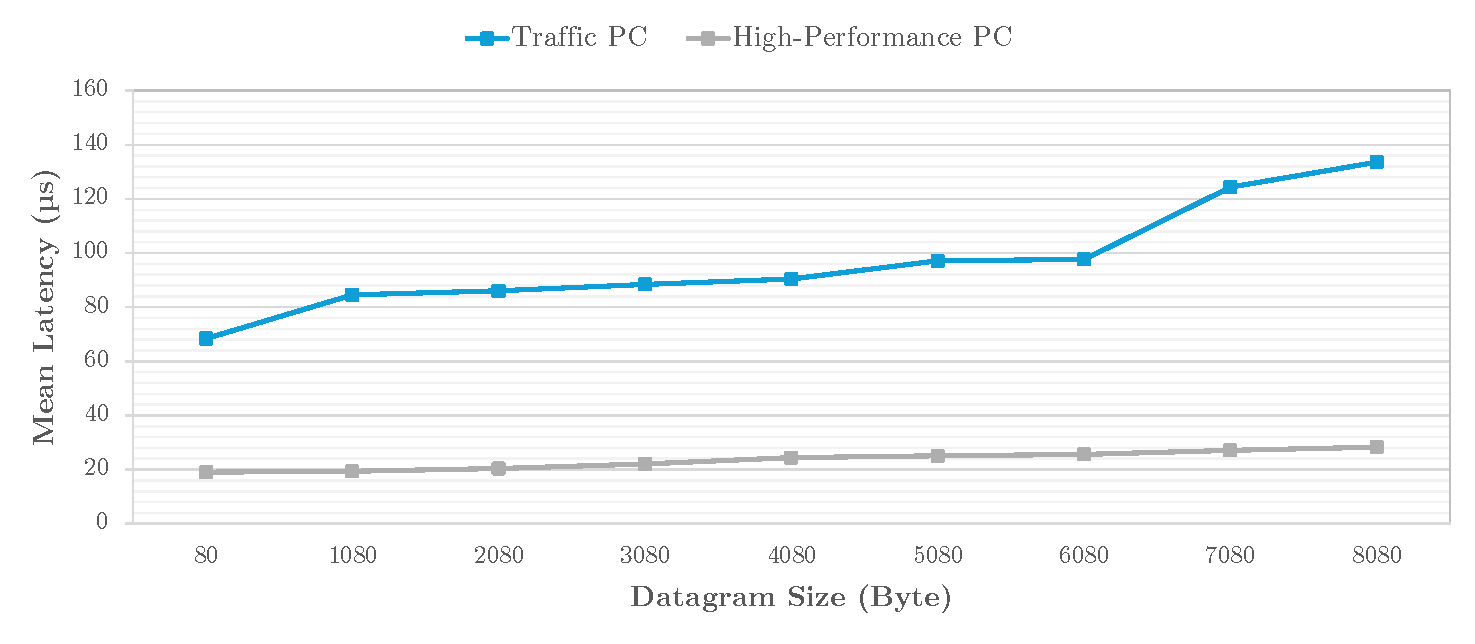
\includegraphics[width=1\textwidth]{figures/performance/d_6a.pdf}
  }
  \subcaptionbox{Direction 'R'\label{fig:TrafficMean:b}}{%
    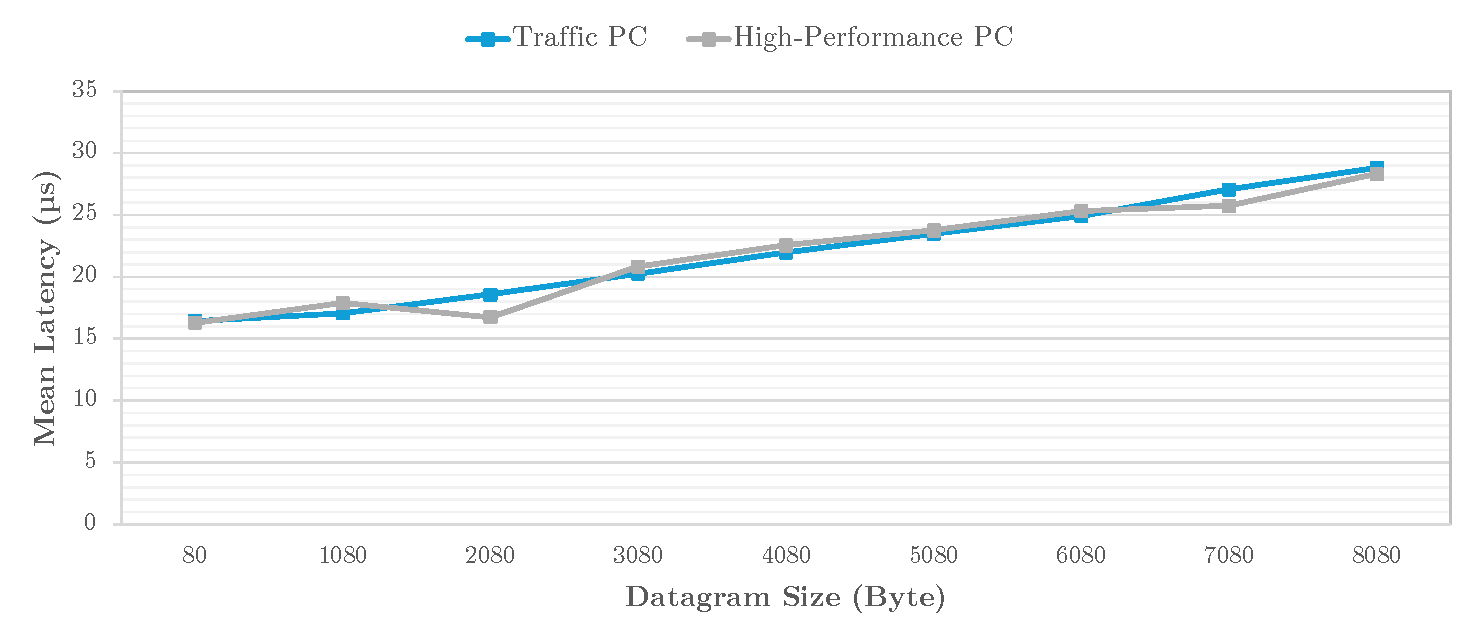
\includegraphics[width=1\textwidth]{figures/performance/d_6b.pdf}
  }
  \caption{Mean Latency by Datagram Size and System under Test (Campaign 'Tests using the System under Test with a Traffic PC').}
  \label{fig:TrafficMean}
\end{figure}

Regarding the mean latency in Direction 'H' with a traffic PC in the system under test, shown in Figure \ref{fig:TrafficMean:a}, it can be observed that it is 108.79 µs on average. This is 76\% higher than in the tests with a High-Performance PC. In direction 'R', shown in figure \ref{fig:TrafficMean:b}, the average mean latency is 24.8 µs, which is almost the same as the average latency measured in the tests with a High-Performance PC. In both directions, there is an increase in latency as the datagram size increases.

\subsubsection{Classification of Results}
The test campaign examined the latency of UDP communication with a Traffic PC in the setup and compared it to a setup with a High-Performance PC.

It was found that the latency in direction "H" is higher for communication between the iHawk and a Traffic PC than for communication between the iHawk and a High-Performance PC. This applies to both the worst-case and mean latency. In contrast, in the 'R' direction, a significantly lower worst-case latency and a comparably high average latency are observed.


\subsection{Tests with additional Load}
\subsubsection{Motivation and Context}
The purpose of this test campaign is to analyze and compare latency under different load situations.

One load situation is to stress all participating computer systems. For this purpose, the realistic load scenario described in Table \ref{tab:realpc} is used. The number and intensity of the stress-ng stressors remain the same. However, no network stressors are used as the focus of this load scenario is on the computer systems.

Additionally, the overall system is subjected to network load. The TestSuite is utilized to generate maximum network load through UDP communications with a datagram size of 8900 bytes and a maximum bandwidth of 10 GBit/s between the iHawk in the center and all participating computer systems of the topology used. This is comparable to the load in the reliability test with the iHawk in the center (refer to Figure \ref{fig:topoihawknaming}). No additional network load is generated on the communication channel whose latency is being measured.

The tests were conducted using UDP sockets and datagram sizes ranging from 80 to 8080 bytes in increments of 1000 bytes. A cycle time of 0 µs and a test duration of 60 seconds were utilized. Only the system under test with the High-Performance PC was evaluated.

\subsubsection{Results}
\paragraph{Worst-Case Latency}

\begin{figure}[h!]
  \centering
  \subcaptionbox{Direction 'H'\label{fig:StressWc:a}}{%
    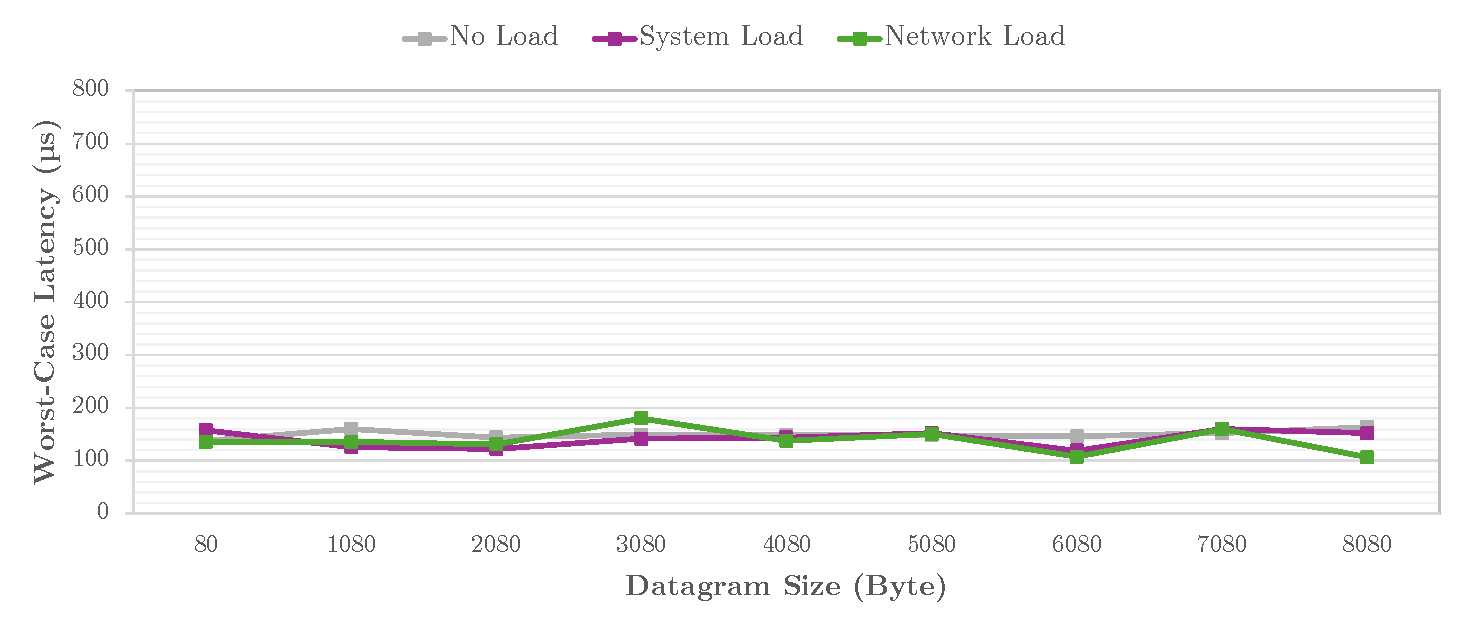
\includegraphics[width=1\textwidth]{figures/performance/d_7a.pdf}
  }
  \subcaptionbox{Direction 'R'\label{fig:StressWc:b}}{%
    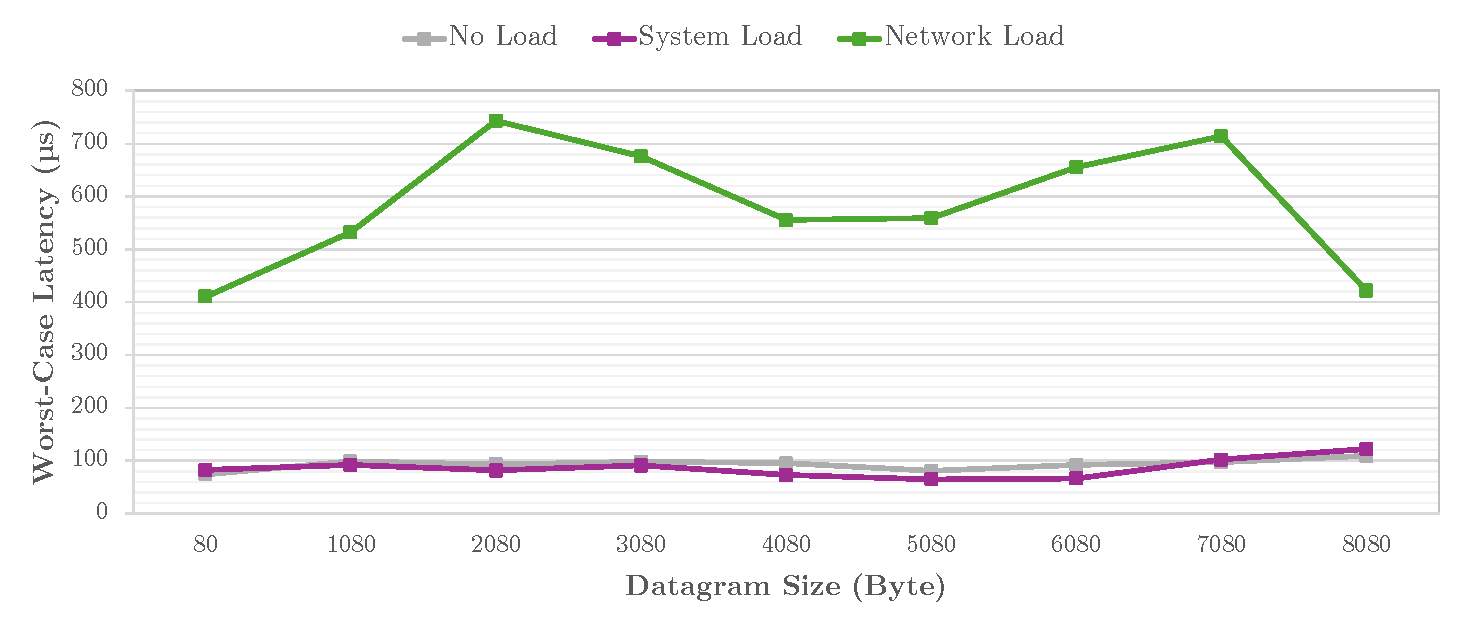
\includegraphics[width=1\textwidth]{figures/performance/d_7b.pdf}
  }
  \caption{Worst-Case Latency by Datagram Size and Load Scenario with the System under Test with a High-Performance PC (Campaign 'Tests with additional Load').}
  \label{fig:StressWc}
\end{figure}

Figure \ref{fig:StressWc} displays the worst-case latency under additional system and network load in directions 'H' and 'R' and compares it to the worst-case latency without additional load.

The realistic scenario causes a CPU utilization of 19.5\% on the iHawk and 47.8\% on the High-Performance PC during the test. In both directions, the worst-case latency remains unaffected by the system load from the realistic scenario. The worst-case latency values are similar to those without additional load.

A network load in direction 'H' (Center to Endpoint) also causes only a small increase in worst-case latency compared to the test with no additional load. The worst-case latency in this direction is 180 µs.

However, in direction 'R' (Endpoint to Center), the network load causes a significant increase in worst-case latency, as shown in Figure \ref{fig:StressWc:b}. The maximum value, measured in tests with a datagram size of 2080 bytes, is 742.73 µs. This increase is due to the high network load on the iHawk in the center. In addition to the measured communication, the system is loaded on 7 other channels with bidirectional communication and an average throughput of 9.68 GBit/s per direction. This high load is causing additional latency during processing in the receiving system.

\paragraph{Mean Latency}
When both computer systems were stressed with the realistic load scenario, average latencies were observed in both directions that were comparable to the tests without load. This also applies to the network load in the direction 'H'.

However, when network load was applied in the 'R' direction, a significantly higher mean latency was observed compared to the test without additional load, as already described for the worst-case latency. The mean latency in this direction was 243.67 µs, which is almost 10 times higher than without additional load (24.67 µs).

\subsubsection{Classification of Results}
The results of the campaign suggest that the latency is not affected by additional system load, such as those from realistic scenarios, which involves CPU load, I/O load, and interrupt load.

When a network load is applied, the worst-case latency increased 4.5 times in the 'R' direction, but remained unchanged in the 'H' direction. This is due to the high network load in the center. It is important to note that this scenario involved applying maximum utilization to all available communication channels.

\subsection{Tests to Investigate the Influence of CPU Affinity}
\subsubsection{Motivation and Context}
This campaign aims to investigate the impact of CPU affinity on latency. Such an investigation has already been done as part of the reliability analysis, so please refer to \ref{chap:AffinityAnalysis} for a detailed description of the goal and motivation of this campaign.

The tests in this campaign examine the CPU affinity option 'enabled' and compare it to no affinity setting. The tests are performed with UDP sockets and datagram sizes from 80 to 8080 bytes in steps of 1000 bytes. A cycle time of 0 µs and a test duration of 60 seconds were used. Only the system under test with the High-Performance PC was used.

\subsubsection{Results}
\paragraph{Worst-Case Latency}

\begin{figure}[h!]
  \centering
  \subcaptionbox{Direction 'H'\label{fig:AffWc:a}}{%
    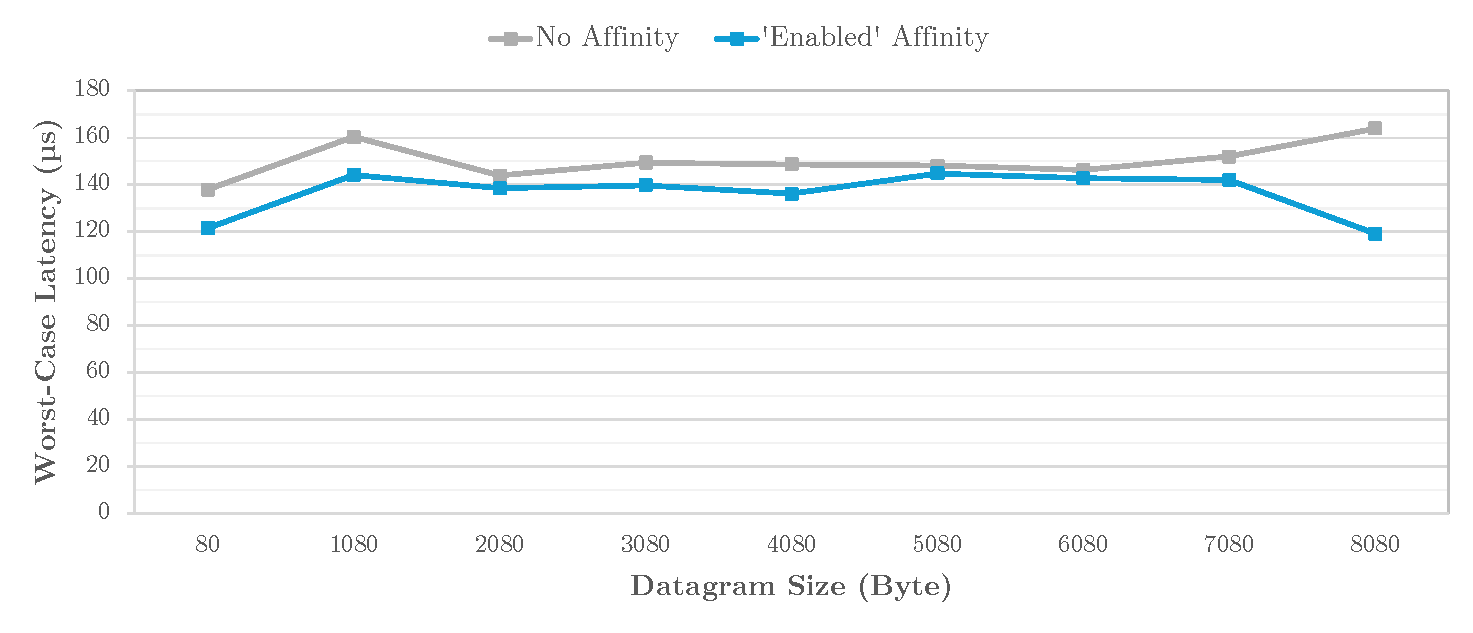
\includegraphics[width=1\textwidth]{figures/performance/d_8a.pdf}
  }
  \subcaptionbox{Direction 'R'\label{fig:AffWc:b}}{%
    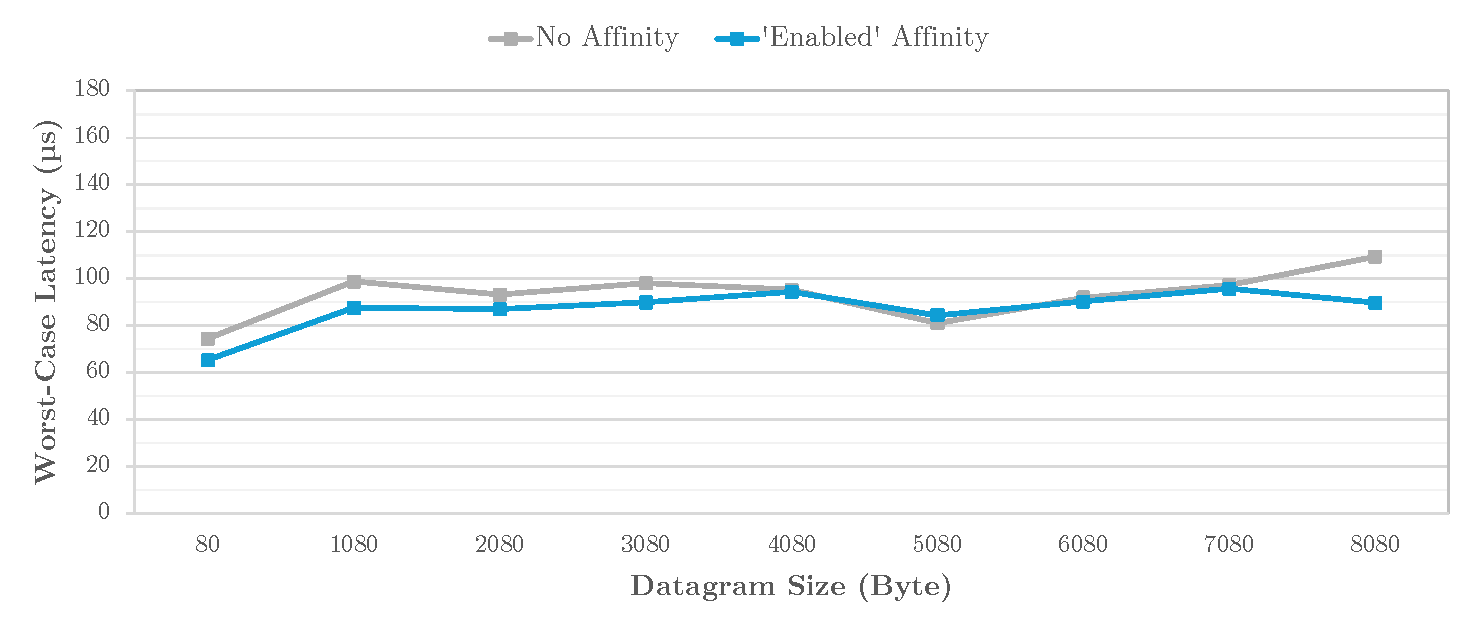
\includegraphics[width=1\textwidth]{figures/performance/d_8b.pdf}
  }
  \caption{Worst-Case Latency by Datagram Size and Affinity Setting with the System under Test with a High-Performance PC (Campaign 'Tests to Investigate the Influence of CPU Affinity').}
  \label{fig:AffWc}
\end{figure}

Figure \ref{fig:AffWc} shows the worst-case latencies for the two investigated CPU affinity settings in both directions, 'H' and 'R'.

In direction 'H' (Center to Endpoint), a maximum worst case latency of 144.76 µs was observed with CPU affinity enabled, which is 11.7\% lower than without CPU affinity enabled. In direction 'R' (Endpoint to Center), a 12.4\% reduction in worst-case latency was observed. Again, as in the previous test campaigns, a higher latency was observed in direction 'H' than in direction 'R'.

It can be assumed that with configured CPU affinity, the fact that the CPU can access its local resources faster than the resources of the remote CPU has a positive influence on the worst-case latency. However, as explained in \ref{chap:iHawkChar}, accessing resources from the other CPU via the UPI link results in a latency of around 130 ns \cite{setup07}. This is a rather small value compared to the measured latencies of UDP communication, which are in the double to triple-digit microsecond range. A further contribution to the observed lower worst-case latencies could also be fluctuations in the measured results.

\paragraph{Mean Latency}

In both directions a mean latency comparable to the mean latency without CPU affinity could be observed for all datagram sizes with enabled CPU affinity (see Figure \ref{fig:SockTypeWc}, Data Series 'UDP Socket'). The maximum deviation observed was 1 µs.

\subsubsection{Classification of Results}
The campaign results indicate that enabling CPU affinity reduces worst-case latency by over 10\% compared to when CPU affinity is not enabled. However, it is important to note that fluctuations in the measurements may have also contributed to these results, in addition to faster resource access by the application. CPU affinity has no effect on the mean latency.

\subsection{Tests to Investigate the Influence of Interrupt-Moderation}
\subsubsection{Motivation and Context}
The purpose of this campaign is to analyze the latency associated with various interrupt moderation configurations.

Interrupt moderation, which can decrease the number of interrupts generated by the network interface, is described in \ref{chap:InterMod}. When examining reliability under different interrupt moderation settings (see \ref{chap:RelInterMod}), it was found that the options examined did not differ in the number of packet losses, but did vary in CPU utilization.

In addition to the previously used disabled interrupt moderation, the timeout values 62 µs and 84 µs recommended in the Intel Linux Performance Tuning Guide \cite{intermod03} as well as the adaptive interrupt moderation were examined. Tests were conducted using UDP sockets and datagram sizes ranging from 80 to 8080 bytes in increments of 1000 bytes. A cycle time of 0 µs and a test duration of 60 seconds were utilized. The campaign only considered the system under test with the High-Performance PC.

\subsubsection{Results}
\paragraph{Worst-Case Latency}

\begin{figure}[h!]
  \centering
  \subcaptionbox{Direction 'H'\label{fig:IMWc:a}}{%
    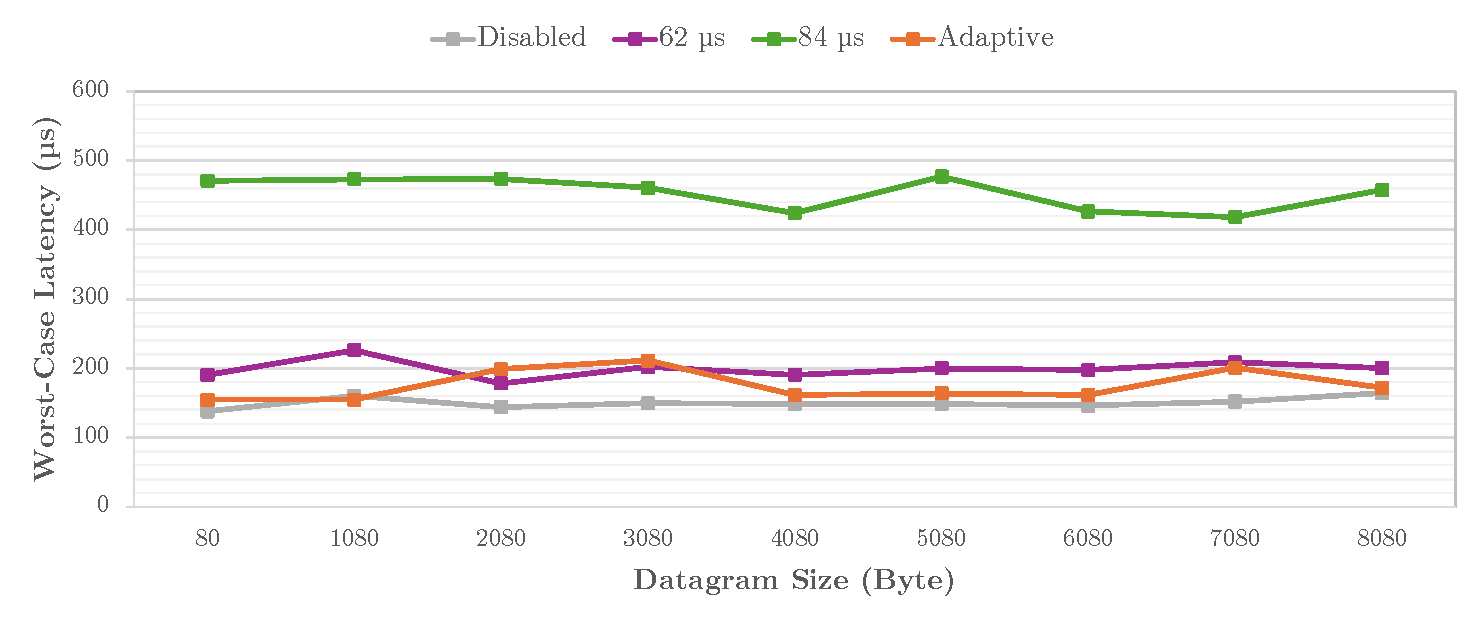
\includegraphics[width=1\textwidth]{figures/performance/d_9a.pdf}
  }
  \subcaptionbox{Direction 'R'\label{fig:IMWc:b}}{%
    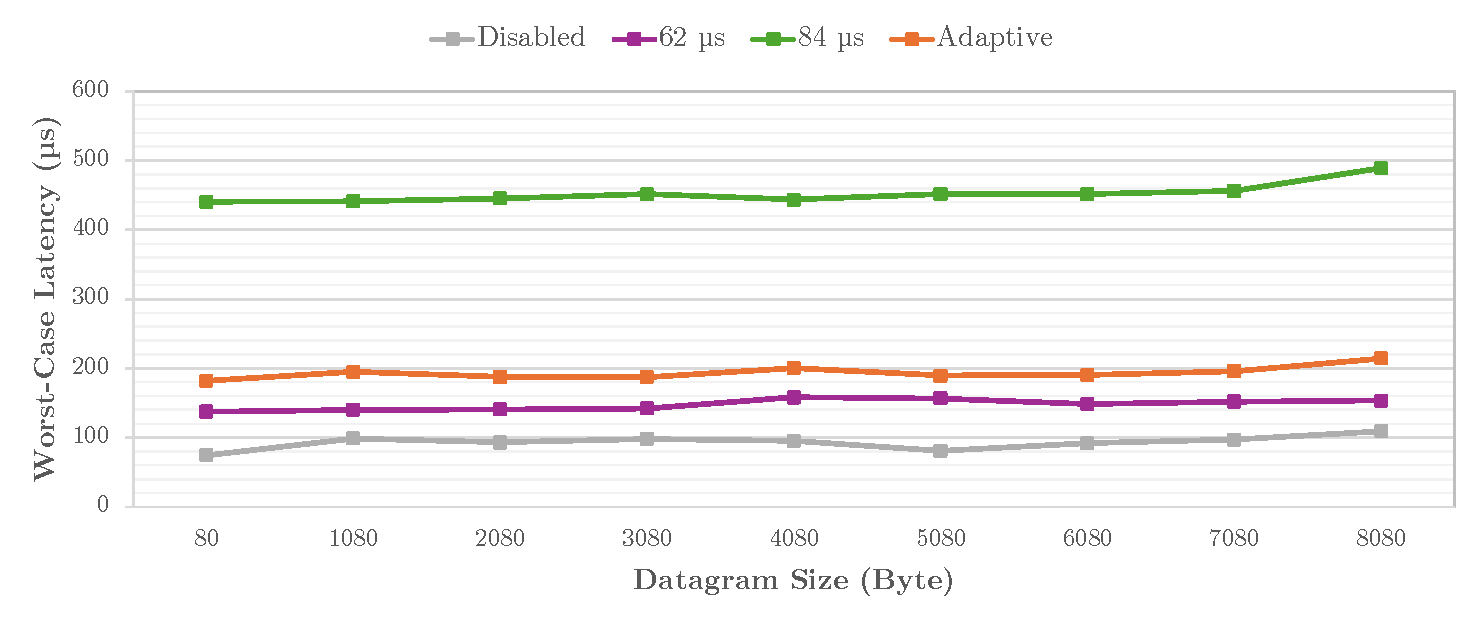
\includegraphics[width=1\textwidth]{figures/performance/d_9b.pdf}
  }
  \caption{Worst-Case Latency by Datagram Size for different Interrupt Moderation Configurations with the System under Test with a High-Performance PC (Campaign 'Tests to Investigate the Influence of Interrupt-Moderation').}
  \label{fig:IMWc}
\end{figure}

Figure \ref{fig:IMWc} displays the worst-case latency for various interrupt moderation configurations in direction 'H' and 'R'.

The highest worst-case latency in direction 'H' is observed with interrupt moderation set to a timeout of 84 µs, with a maximum of 476.73 µs. The setting with a timeout value of 62 µs has a worst-case latency of 226.05 µs, which is considerably lower. With adaptive interrupt moderation, a worst case latency of 211.16 µs was observed with a datagram size of 3080 bytes. However, when interrupt moderation was disabled, the lowest worst-case latency was observed at 163.97 µs. Figure \ref{fig:IMWc:a} shows the worst-case latency against datagram size for all interrupt moderation configurations. No clear trend can be identified.

In direction 'R', the highest worst-case latency of 488.94 µs is also observed with interrupt moderation set to a timeout value of 84 µs. Adaptive interrupt moderation has a worst-case latency of 214.11 µs in this direction, which is similar to the value in the 'H' direction. With a timeout value of 62 µs, a worst-case latency of 158.13 µs is measured, while the lowest worst-case latency of 109.31 µs is also observed in this direction with disabled interrupt moderation. Similar to previous campaigns, the worst-case latency is lower in the 'R' direction compared to the 'H' direction, except for adaptive interrupt moderation.

The finding that the timeout values have a higher worst-case latency than the disabled interrupt moderation was expected, since interrupt moderation, as described in \ref{chap:InterMod}, delays the generation of interrupts.  The worst-case latency in both directions for adaptive interrupt moderation ranges from 210 µs to 215 µs. Based on the test results, no clear dependency between datagram size and latency can be recognized for this configuration, although the description of the functionality (see \ref{chap:InterMod}) suggests otherwise.

\paragraph{Mean Latency}

Figure \ref{fig:IMean} shows the mean latency based on datagram size and interrupt moderation configuration.

\begin{figure}[h!]
  \centering
  \subcaptionbox{Direction 'H'\label{fig:IMean:a}}{%
    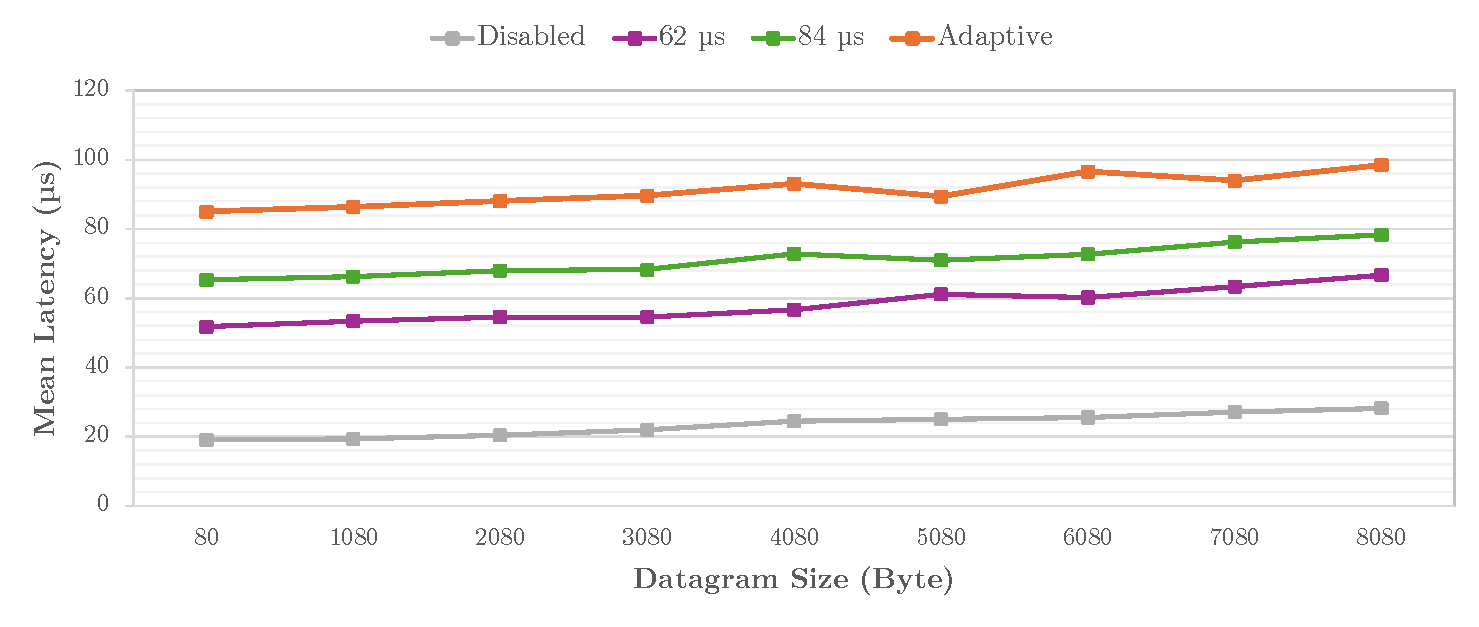
\includegraphics[width=1\textwidth]{figures/performance/d_10a.pdf}
  }
  \subcaptionbox{Direction 'R'\label{fig:IMean:b}}{%
    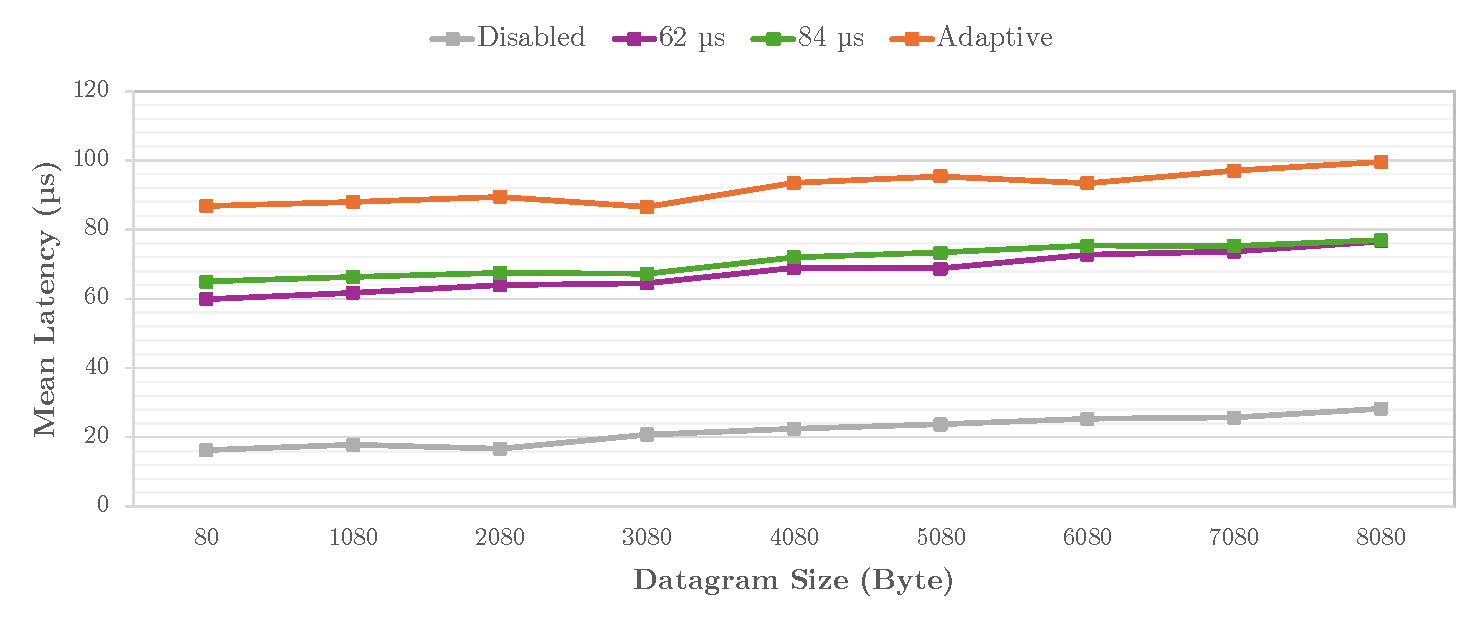
\includegraphics[width=1\textwidth]{figures/performance/d_10b.pdf}
  }
  \caption{Mean Latency by Datagram Size for different Interrupt Moderation Configurations with the System under Test with a High-Performance PC (Campaign 'Tests to Investigate the Influence of Interrupt-Moderation').}
  \label{fig:IMean}
\end{figure}

The results show that activating interrupt moderation with a timeout value of 62 µs increases the average latency in direction 'H' by more than two times and in direction 'R' by more than three times. As expected, the configuration with a timeout value of 84 µs has an even higher mean latency.

The mean latency for adaptive interrupt moderation is 103 µs in both directions, making it the highest observed mean latency. Figure \ref{fig:IMean} shows a slight increase in mean latency with increasing datagram size. The interrupt moderation rate for adaptive interrupt moderation is determined by the number of connections and packet size. In this test with a low number of connections, a high number of interrupts per second should be configured for low latency \cite{intermod04}. However, this behavior cannot be confirmed in the performed tests, as the measured average latency is the highest compared to the other options examined. One possible reason for this could be the test duration, which may be too short for the adaptive interrupt moderation to configure itself.

\subsubsection{Classification of Results}
The results indicate that latency is at its lowest when interrupt moderation is deactivated. Additionally, the campaign presents the expected worst-case and mean latencies for interrupt moderation configurations with timeout values of 62 µs and 84 µs.

The highest latencies were measured with an adaptive interrupt configuration. However, the configuration changes due to factors such as the number of packets, packet size, or number of connections. As a result, the measured latency may fluctuate, making this option unsuitable for use in a distributed Test Support System.

\subsection{Tests with the Intel X540-T2 Network Interface}
\subsubsection{Motivation and Context}

This campaign aims to investigate the latency of the Intel X540-T2 network interfaces in both iHawk and HPC1. The reliability of these interfaces has already been examined in \ref{chap:IntelRel540}, where no difference was found compared to the currently used Intel X710-T2L.

The test also employed the settings from the Intel Linux Performance Tuning Guide (see \cite[intermod03]) for the Intel X540-T2 network interfaces. This means for example that interrupt moderation is disabled.

The test mode used for this campaign was the same as in the previous campaigns. This involved the use of UDP sockets and datagram sizes ranging from 80 to 8080 bytes, with a cycle time of 0 µs and a test duration of 60 seconds. Only the system under test with the High-Performance PC was utilized.

\subsubsection{Results}
\paragraph{Worst-Case Latency}

\begin{figure}[h!]
  \centering
  \subcaptionbox{Direction 'H'\label{fig:540Wc:a}}{%
    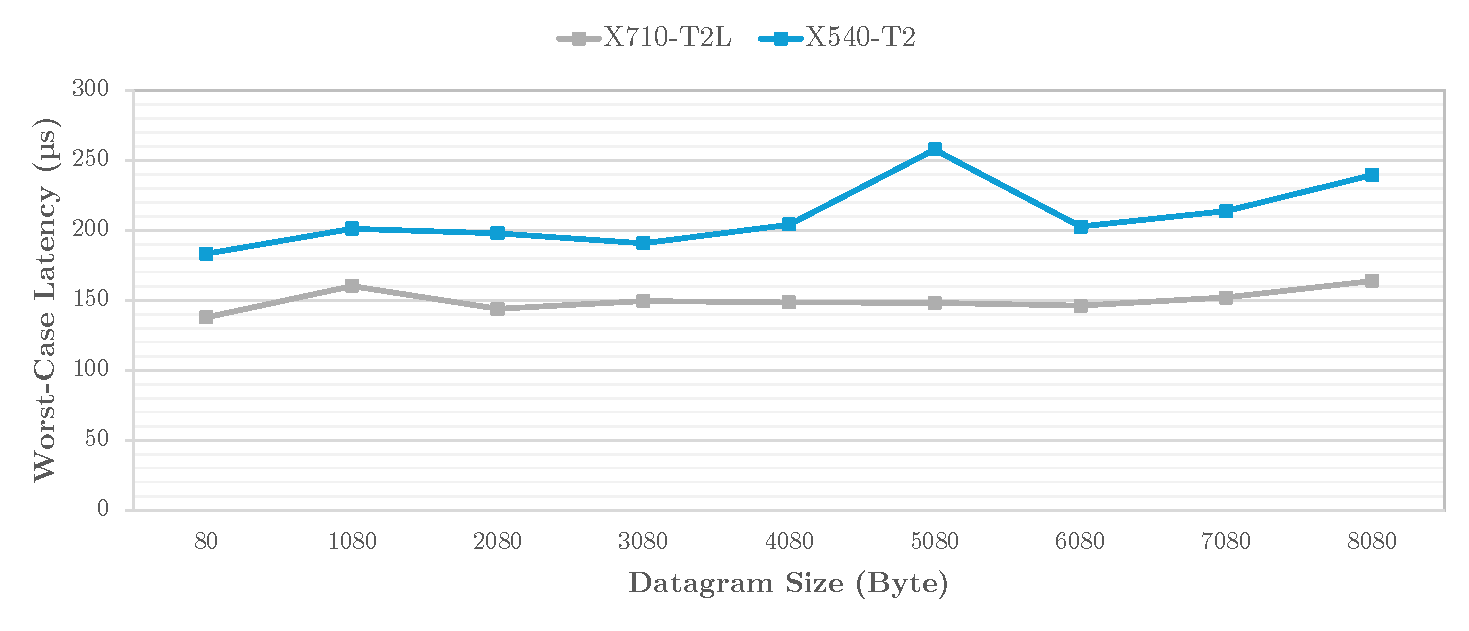
\includegraphics[width=1\textwidth]{figures/performance/d_11a.pdf}
  }
  \subcaptionbox{Direction 'R'\label{fig:540Wc:b}}{%
    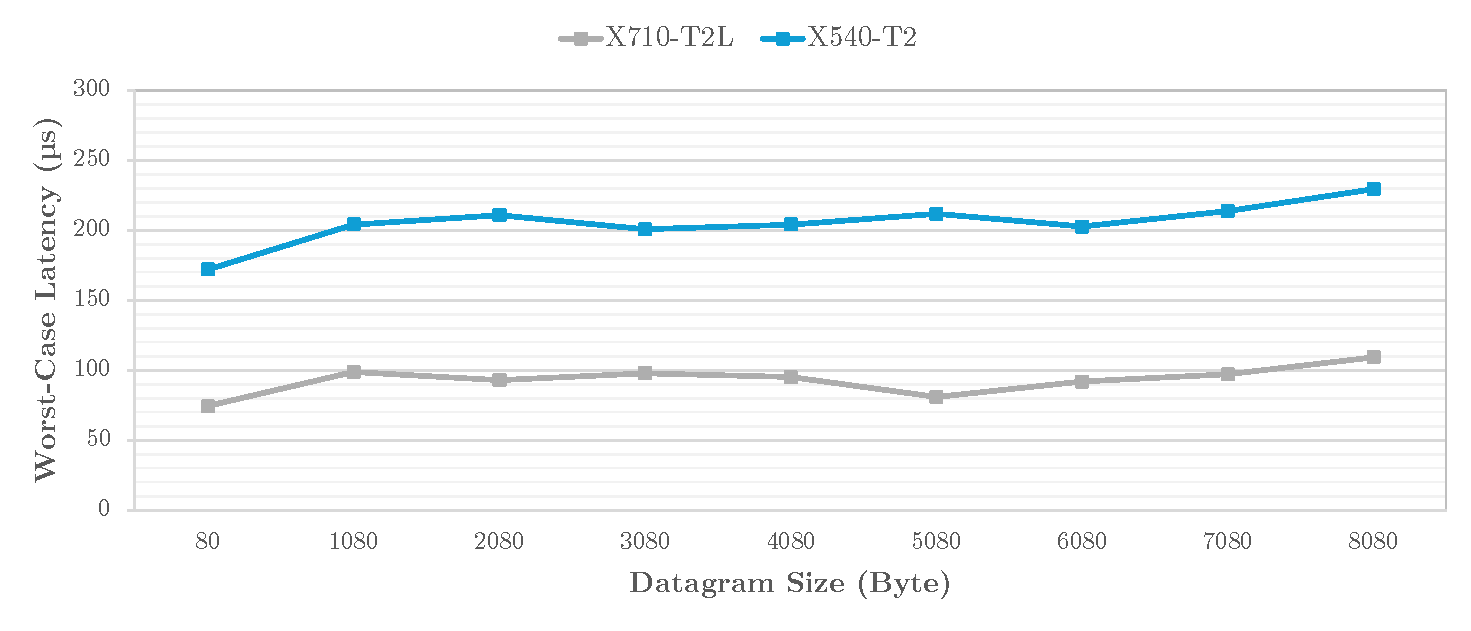
\includegraphics[width=1\textwidth]{figures/performance/d_11b.pdf}
  }
  \caption{Worst-Case Latency by Datagram Size of the Intel X540-T2 Network Interface compared with the Intel X710-T2L Network interface (Campaign 'Tests with the Intel X540-T2 Network Interface').}
  \label{fig:540Wc}
\end{figure}

Figure \ref{fig:540Wc} shows the worst-case latency when using the Intel X540-T2 network interfaces compared to the Intel X710-T2L network interfaces in both directions.

The results show that the worst-case latency is greater when using the Intel X540-T2 in both directions compared to the Intel X710-T2L. Across all datagram sizes, the worst-case latency is 257.79 µs in direction 'H' and 229.56 µs in direction 'R'.

The higher worst-case latencies with the same configuration with the Intel X540-T2 can be attributed to the fact that the network interface itself is older compared to the Intel X710-T2L. Additionally, the network interfaces use different drivers (see Table \ref{tab:drivernic}), which also affects the latency.

\paragraph{Mean Latency}

\begin{figure}[h!]
  \centering
  \subcaptionbox{Direction 'H'\label{fig:540Mean:a}}{%
    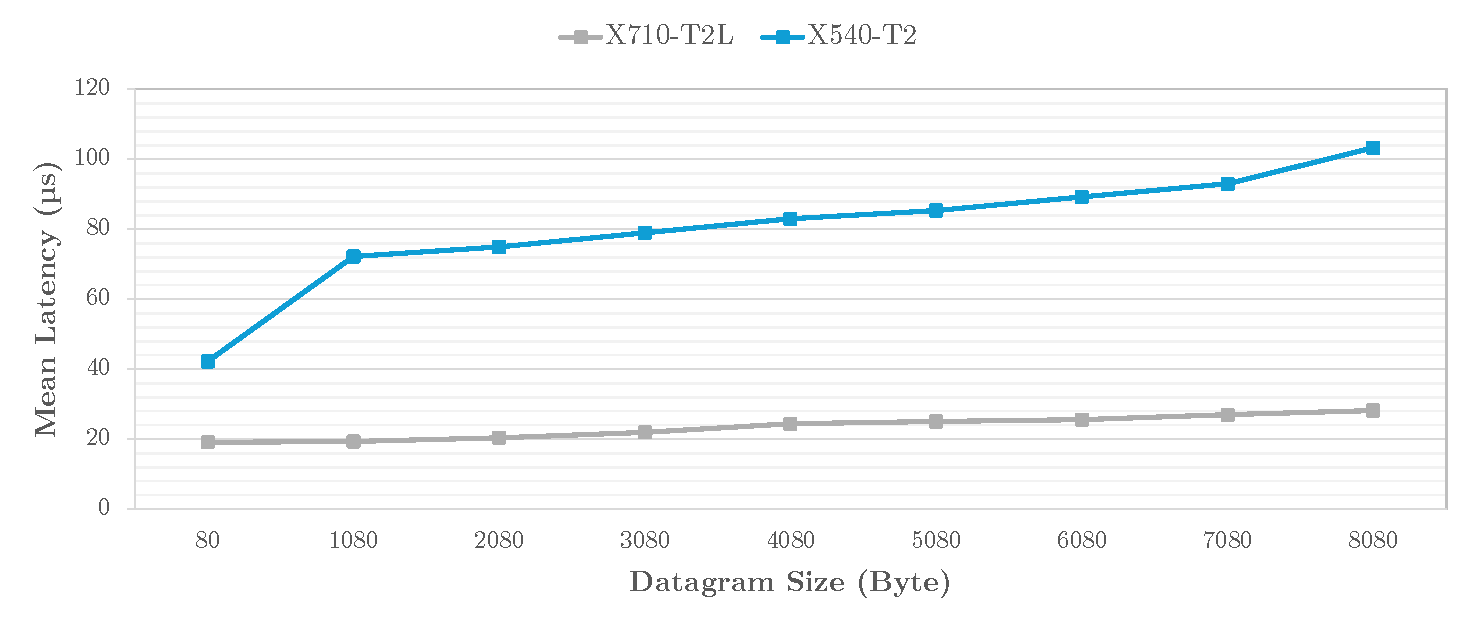
\includegraphics[width=1\textwidth]{figures/performance/d_12a.pdf}
  }
  \subcaptionbox{Direction 'R'\label{fig:540Mean:b}}{%
    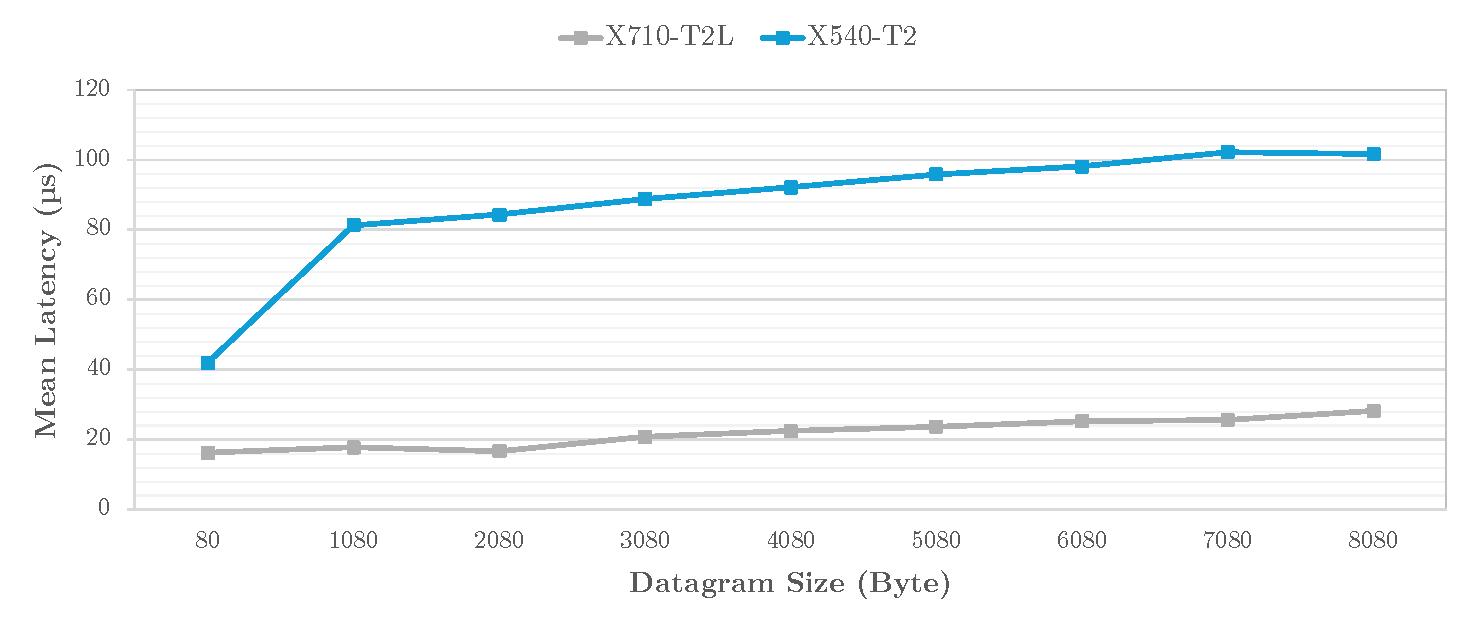
\includegraphics[width=1\textwidth]{figures/performance/d_12b.pdf}
  }
  \caption{Mean Latency by Datagram Size of the Intel X540-T2 Network Interface compared with the Intel X710-T2L Network interface (Campaign 'Tests with the Intel X540-T2 Network Interface').}
  \label{fig:540Mean}
\end{figure}

Figure \ref{fig:540Mean} displays a comparison of the mean latency of the Intel X540-T2 and Intel X710-T2L network interfaces. The mean latency in both directions, 'H' and 'R', increases with larger datagram sizes and is on average about 90.30 µs in the 'H' direction and 98.34 µs in the 'R' direction.

It is noticeable that with a datagram size of 80 bytes, the average latency in both directions has a value of about 42 µs and increases significantly with a datagram size of 1080 bytes. These differences are not observable when using the Intel X710-T2L network interfaces with small datagrams.

\subsubsection{Classification of Results}
The campaign has demonstrated that the Intel X540-T2 network interfaces exhibit significantly higher latencies than the Intel X710-T2L network interfaces with the same configuration. This applies to both worst-case and mean latencies. Therefore, when using these network interfaces in the distributed Test Support System, a higher latency should be expected.

\section{Insights}
The analysis of performance has revealed the anticipated latencies of a UDP communication on the application level. The lowest latencies are to be expected when communication is between the iHawk and a High-Performance PC. However, when communicating systems similar to Traffic PCs, higher latencies should be expected in some cases.

The study also examined latencies with Raw sockets and Packet sockets, in addition to UDP sockets. The results indicate that Packet sockets have lower latency than the other socket types, but sometimes packets do not arrive in the order in which they were sent.

Further the investigation analyzed the impact of different load scenarios on the computer systems involved. The study found that exceptionally high network load on the receiving side increases the worst-case latency by a factor of ten. In contrast, a system with similar load to that in the Test Support System does not show an increase in latency.

The study investigated the impact of CPU affinity on multi-socket systems and found that it has a minor effect on latency. Also the latencies can be expected with different interrupt moderation options are presented. As expected, the lowest latency was observed when interrupt moderation was disabled. 

Additionally, the study examined the latency of the Intel X540-T2 network interface and found it to be higher than that of the newer Intel X710-T2L network interface.

